\documentclass{article}

\usepackage{graphicx}
\usepackage{tikz}
\usepackage{tikzsymbols}
\usetikzlibrary{calc,patterns,shapes.geometric}
\pagestyle{empty}
\usepackage[margin=0pt]{geometry}
\geometry{papersize={14in,12in}}

\def\centerarc[#1](#2)(#3:#4:#5){\draw[#1] ($(#2)+({#5*cos(#3)},{#5*sin(#3)})$) arc (#3:#4:#5);}

\begin{document}
	\begin{figure}
		\centering
		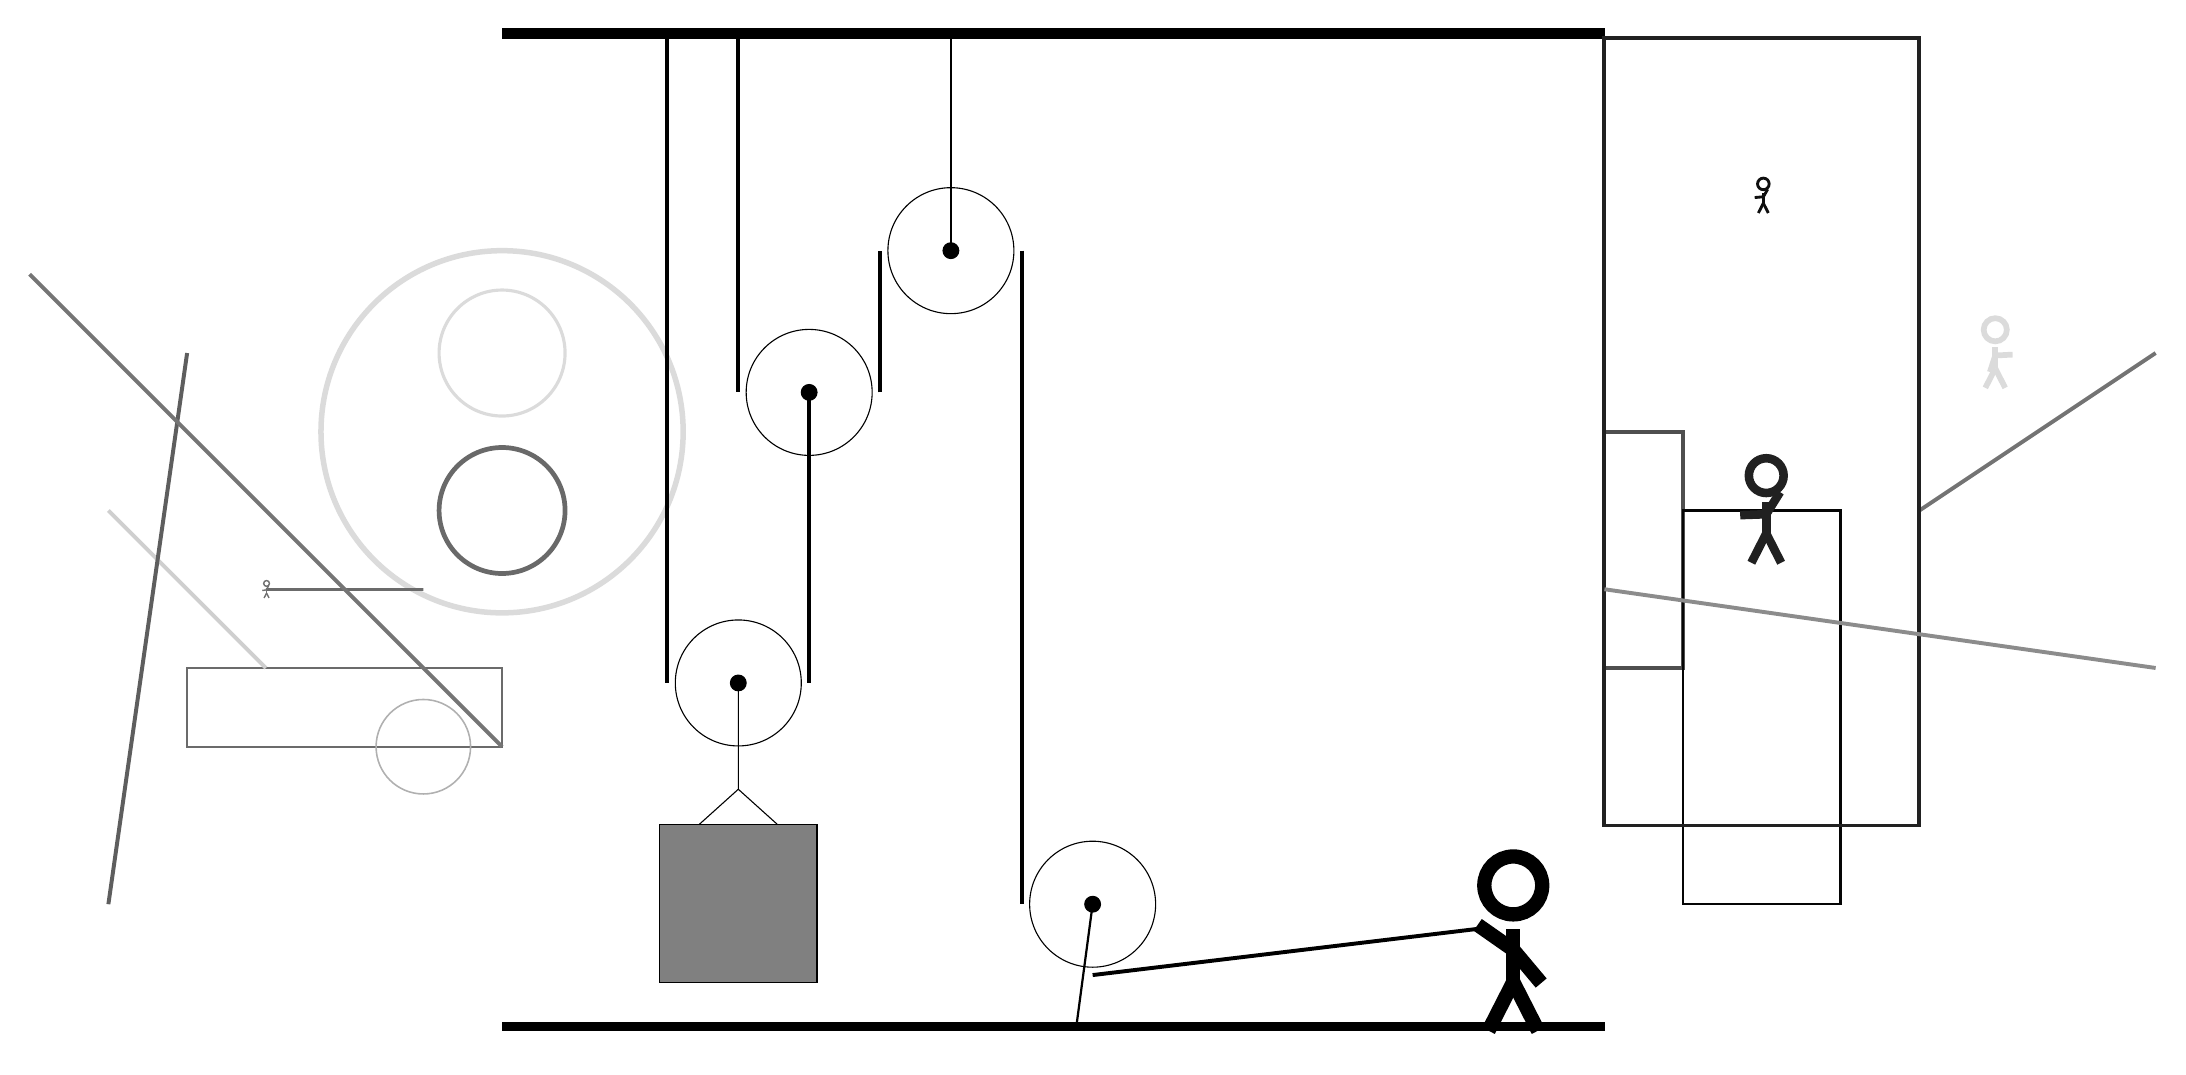
\begin{tikzpicture}
			%%%%% START %%%%%
			
			\draw[fill=black] (-2, 9) rectangle (12, 9.125);
			
			\draw (1, 0.81) circle (0.8);
			\draw[fill=black] (1, 0.81) circle (0.1);
			
			\draw[line width=0.5mm, color=black!55](16, 3) -- (19, 5);
			
			\draw [line width=0.7mm, color=black!14](-2, 4) circle (2.3);
			\draw[line width=0.2mm, color=black!58] (-2, 0) rectangle (-6, 1);
			\draw[line width=0.5mm, color=black!69] (12, 4) rectangle (13, 1);
			\draw [line width=0.4mm, color=black!14](-2, 5) circle (0.8);
			\draw[line width=0.3mm, color=black!98] (13, -2) rectangle (15, 3);
			\node[line width=0.6mm, color=black!87] at (14, 3) {\Strichmaxerl[6][2][58]};
			\draw[line width=0.5mm, color=black!19](-7, 3) -- (-5, 1);
			\draw[line width=0.4mm, color=black!58] (-3, 2) rectangle (-5, 2);
			\draw[line width=0.5mm, color=black!63](-7, -2) -- (-6, 5);
			
			\draw[line width=0.5mm, color=black!87] (12, -1) rectangle (16, 9);
			\draw [line width=0.2mm, color=black!31](-3, 0) circle (0.6);
			\node[line width=0.4mm, color=black!94] at (14, 7) {\Strichmaxerl[2][5][60]};
			
			\draw[line width=0.5mm, color=black!45](12, 2) -- (19, 1);
			\draw [line width=0.6mm, color=black!59](-2, 3) circle (0.8);
			\node[line width=0.2mm, color=black!56] at (-5, 2) {\Strichmaxerl[1][8][65]};
			
			\node[line width=0.6mm, color=black!14] at (17, 5) {\Strichmaxerl[4][72][3]};
			\draw[line width=0.5mm, color=black!54](-2, 0) -- (-8, 6);
			
			\draw (1.9, 4.5) circle (0.8);
			\draw[fill=black] (1.9, 4.5) circle (0.1);
			
			\draw (3.7, 6.3) circle (0.8);
			\draw[fill=black] (3.7, 6.3) circle (0.1);
			\draw[thick] (3.7, 6.3) -- (3.7, 9);
			
			\draw (5.5, -2) circle (0.8);
			\draw[fill=black] (5.5, -2) circle (0.1);
			\draw[thick] (5.5, -2) -- (5.3, -3.5);
			
			\draw (1, 0.81) -- (1, -0.54) -- (0.5, -0.99) -- (1.5, -0.99) -- (1, -0.54);
			\draw[fill=black!50] (0, -0.99) rectangle (2, -2.99);
			\draw[line width=0.5mm] (0.1, 9) -- (0.1, 0.81);
			\centerarc[line width=0.5mm](1, 0.81)(180:360:0.9);
			\draw[line width=0.5mm](1.9, 0.81) -- (1.9, 4.5);
			\draw[line width=0.5mm] (1.0, 9) -- (1.0, 4.5);
			\centerarc[line width=0.5mm](1.9, 4.5)(180:360:0.9);
			\draw[line width=0.5mm](2.8, 4.5) -- (2.8, 6.3);
			\centerarc[line width=0.5mm](3.7, 6.3)(0:180:0.9);
			\draw[line width=0.5mm] (4.6, 6.3) -- (4.6, -2);
			\centerarc[line width=0.5mm](5.5, -2)(0:90:-0.9);
			\draw[line width=0.5mm](5.5, -2.9) -- (10.5, -2.3);
			
			\node at (10.8, -2.5) {\Strichmaxerl[10][-35][-50]};
			
			\draw[fill=black] (-2, -3.5) rectangle (12, -3.6);
			
			%%%%% END %%%%%
		\end{tikzpicture}
	\end{figure}	
\end{document}